%! Author = Christoph Renzing
%! Date = 21.04.22

% Preamble
\documentclass[11pt]{PyRollDocs}
\usepackage{textcomp}

\addbibresource{refs.bib}
% Document
\begin{document}

    \title{Lendl's equivalent rectangle method PyRoll Plugin}
    \author{Christoph Renzing}
    \date{\today}

    \maketitle

    This plugin provides the equivalent method after Lendl for calculation of an equivalent rectangle used for spread calculation.


    \section{Model approach}\label{sec:model-approach}

    A common approach for groove rolling is to calculate some equivalent rectangular profile to be able to use spread models for flat rolling in groove rolling.
    This method is valid if the groove design is a simple irregular one.
    For this case, the roll pass is characterized by a change in height that varies across the width, with the caliber having more than one axis of symmetry.
    \textcite{Lendl_1948a, Lendl_1948b, Lendl_1949} proposed a method for calculation of an equivalent rectangle using the incoming profile of the roll pass and the groove used in the pass.
    The method can be divided into four different steps witch are explained in detail in the following subsections.

    \begin{itemize}
        \item Calculation of intersection points between the incoming profile and groove
        \item Calculation of Lendl Area of the roll pass
        \item Calculation of Lendl width of the roll pass
        \item Calculation of Lendl height
    \end{itemize}

    \subsection{Calculation of intersection points}\label{subsec:intersection-points}
    As for groove and profile contour lines are so called \texttt{LineString} objects provided by the shapely package published by \textcite{shapely2007}.
    For calculation of intersection points between incoming profile and groove the shapely method \texttt{intersection} is used.
    This method returns the points where two lines intersect each other.
    As an example the following figure~\ref{fig:lendl-intersection-points} show's the intersection points of an incoming round profile and an oval groove.

    \begin{figure}
        \centering
        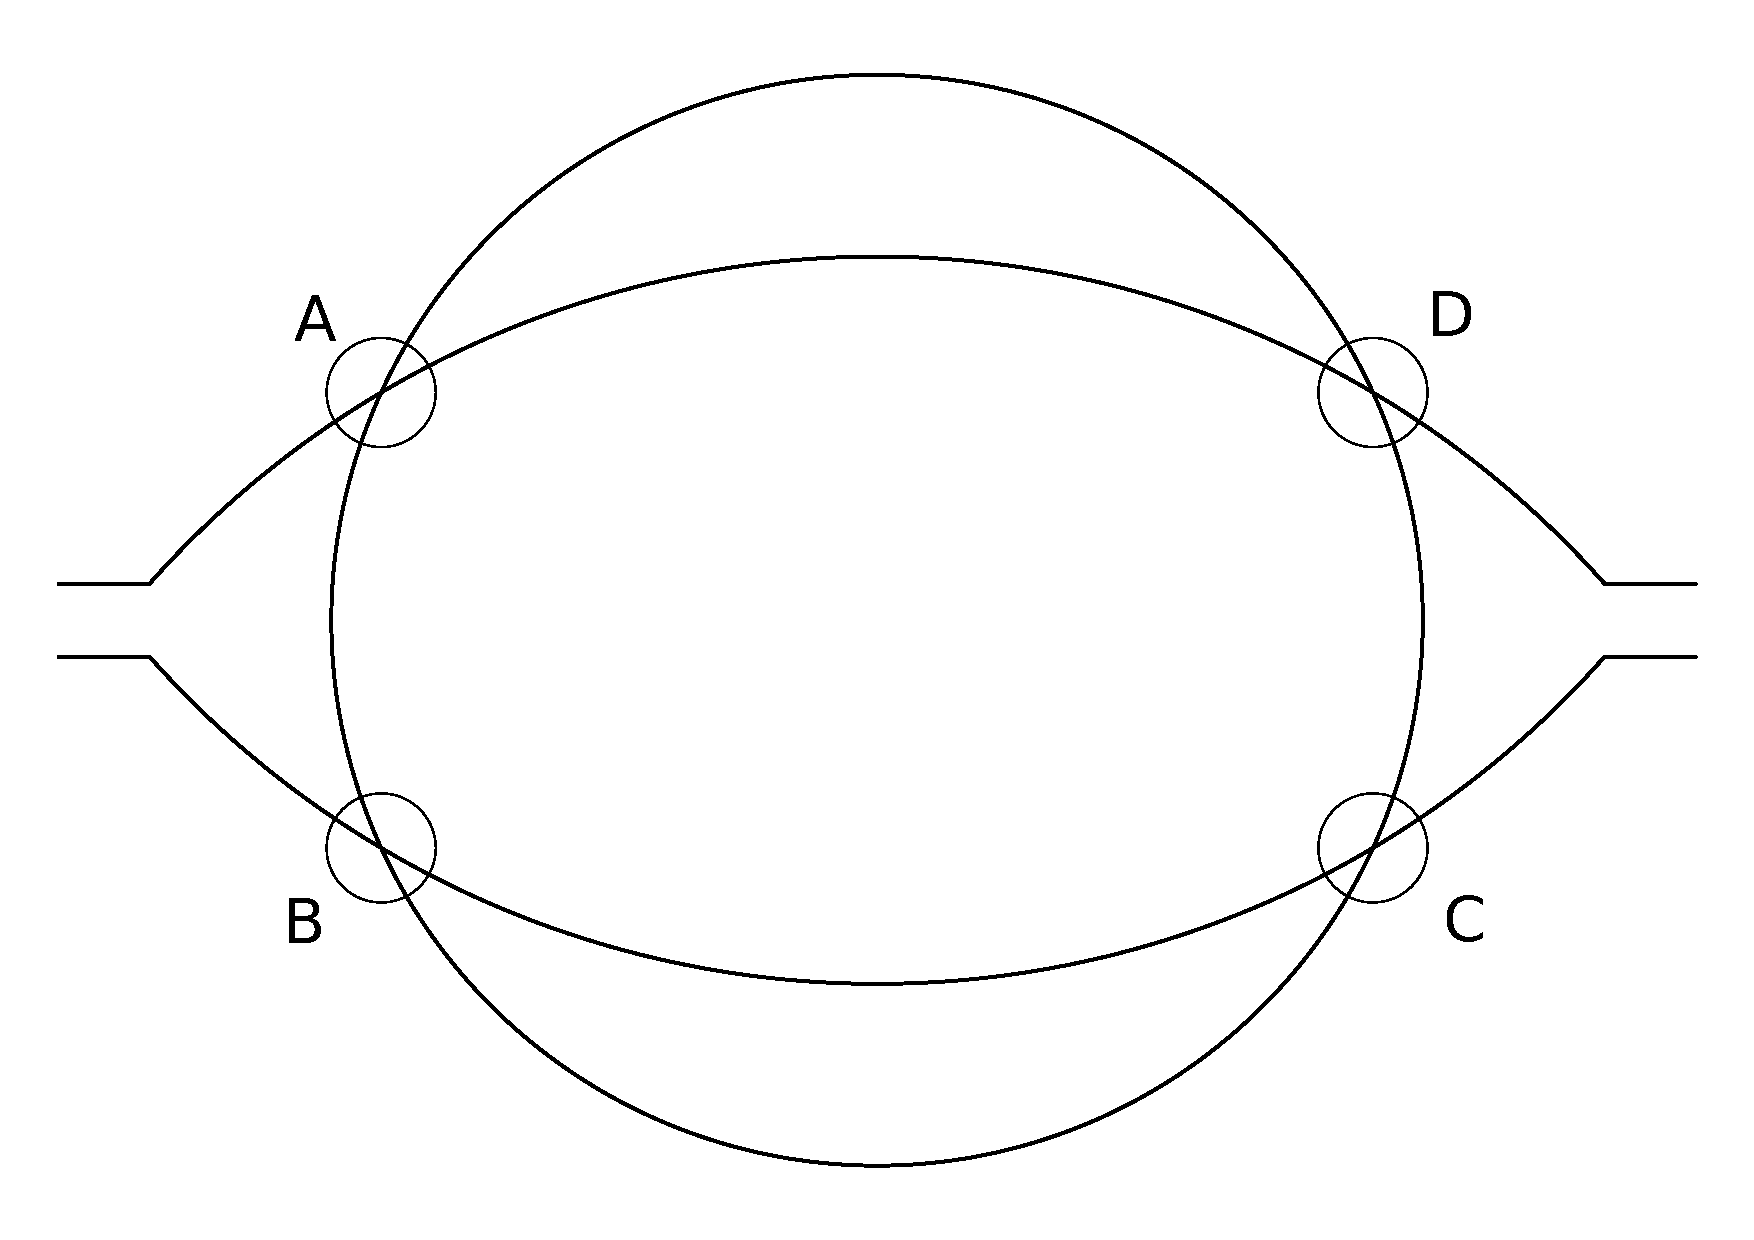
\includegraphics[width=.7\linewidth]{lendl-intersection}
        \caption{Intersection points A to D for a round - oval roll pass}
        \label{fig:lendl-intersection-points}
    \end{figure}

    \subsection{Calculation of Lendl's area for incoming profile and roll pass}\label{subsec:lendl-areas}
    Lendl's area for the incoming profile ($A_{0,L}$) is the area under direct pressure from the work roll.
    For the groove, Lendl's area is the area under direct pressure inside the groove ($A_{1,L}$).
    As an example Lendl areas for the already shown round - oval roll pass are shown in figure~\ref{fig:lendl-areas}.
    One can also derive the following condition for these areas in relation to the total area of the incoming ($A_{0}$) and outgoing profile areas ($A_{1}$).

    \begin{subequations}
        \begin{equation}
            A_{0,L} < A_{0}
            \label{eq:incoming-area-ratio}\\
        \end{equation}
        \begin{equation}
            A_{1,L} < A_{1}
            \label{eq:outgoing-area-ratio}
        \end{equation}
    \end{subequations}

    \begin{figure}[ht]
        \centering
        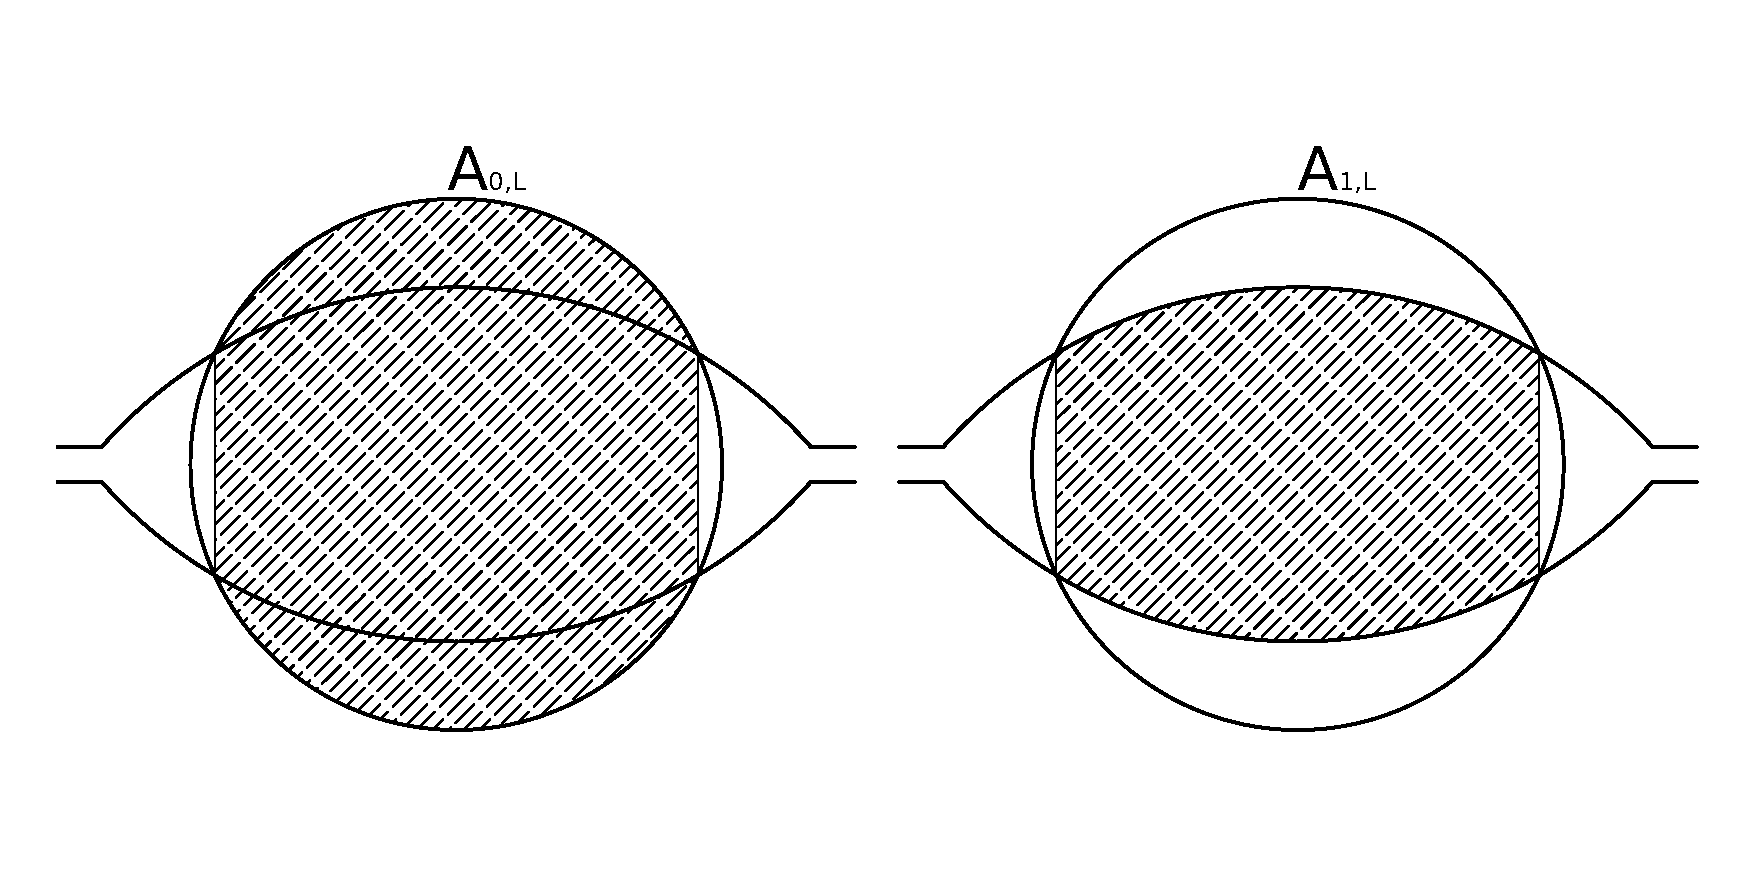
\includegraphics[ width=15cm,
            height=5.5cm,
            keepaspectratio,]{lendl-area}
        \caption{Lendl areas for a round - oval roll pass}
        \label{fig:lendl-areas}
    \end{figure}

    \newpage

    \subsection{Calculation of Lendl's width}\label{subsec:lendl-width}
    Lendl's width is calculated as the distance of the vertical connection between the intersection points A and B and C and D.
    For calculation the shapely method \texttt{distance} is used.

    \subsection{Calculation of Lendl's equivalent height}\label{subsec:lendl-height}
    Calculation of Lendl's equivalent height is carried out by dividing Lendl's area through Lendl's width.
    The resulting height is used as the height of the equivalent rectangle used in the equivalent flat roll pass.
    As for the initial width of the incoming profile \textcite{Mauk_Kopp_1982} stated that using the maximum width of the incoming profile is suitable


    \section{Usage instructions}\label{sec:usage-instructions}

    The plugin can be loaded under the name \texttt{pyroll\_lendl\_equivalent\_method}.

    An implementation of the hooks \lstinline{lendl_width}, \lstinline{lendl_initial_area} and \lstinline{lendl_final_area}
    for calculation the values for $b_L$, $A_{0,L}$ and $A_{1,L}$ is provided on the \lstinline{RollPass}.
    Several additional hooks on \lstinline{RollPass} are defined, which are used for calculation, as listed in \autoref{tab:hookspecs}.
    On the \lstinline{RollPass.InProfile} the hook \lstinline{equivalent_rectangle} calculates the corresponding equivalent rectangle for the profile.
    The same hook can be called on the \lstinline{RollPass.OutProfile} providing the same usability.

    \begin{table}
        \centering
        \caption{Hooks specified by this plugin.}
        \label{tab:hookspecs}
        \begin{tabular}{ll}
            \toprule
            Hook name                                  & Meaning                                                     \\
            \midrule
            \texttt{right\_contour}                    & right contour of the profile after rotation                 \\
            \texttt{left\_contour}                     & left contour of the profile after rotation                  \\
            \texttt{upper\_left\_intersection\_point}  & upper left intersection point $A$ in~\ref{fig:lendl-areas}  \\
            \texttt{upper\_right\_intersection\_point} & upper right intersection point $B$ in~\ref{fig:lendl-areas} \\
            \texttt{lower\_left\_intersection\_point}  & lower left intersection point  $D$ in~\ref{fig:lendl-areas}   \\
            \texttt{lower\_right\_intersection\_point} & lower right intersection point $C$ in~\ref{fig:lendl-areas} \\
            \texttt{left\_lendl\_width\_boundary}      & connection line between $A$ and $B$                         \\
            \texttt{right\_lendl\_width\_boundary}     & connection line between $D$ and $C$                         \\
            \texttt{lendl\_width}                      & Lendl's width $b_L$                                         \\
            \texttt{lendl\_initial\_area}              & Lendl's initial area $A_{0,L}$                              \\
            \texttt{lendl\_final\_area}                & Lendl's width $A_{1,L}$                                     \\
            \texttt{equivalent\_rectangle}             & Equivalent rectangle of the profile or groove               \\

            \bottomrule
        \end{tabular}
    \end{table}

    \printbibliography


\end{document}